\section{问题四的模型建立与求解}

问题四采用附件 2 给定的半径轨迹 $R(t)$，假设均匀径向收缩、轴向长度不变且干骨架无损失。令材料坐标 $\xi=r/R(t)$，则计算域固定为 $0\le\xi\le1$。由材料守恒，收缩速度为 $v_r=(\dot R/R)r$；物质导数中的运动项与坐标变换项抵消，得到
\[
 U_t=\frac{1}{R(t)^2\xi}\partial_\xi(\xi D(U,\Theta)U_\xi),\qquad
 \rho(U)c_p(U)\Theta_t=\frac{1}{R(t)^2\xi}\partial_\xi(\xi k(U)\Theta_\xi).
\]
表面条件保留半径尺度：$-k\Theta_\xi/R=h(\Theta_s-T_\infty)$、$-DU_\xi/R=k_m(U_s-C_e)$。因此坐标变换固定了网格，但没有消除收缩对内部传递和表面阻力的影响。

附录 4 的 $\rho,c_p,k,D$ 整组替换，采用与前述各问一致的 Kirchhoff 水分通量、Robin 半控制体和 BDF 推进。连续事件定义为
\[
 M(t)=\max_{0\le\xi\le1}C_h(\xi,t),\qquad t_* =\inf\{t:M(t)\le0.15\}.
\]
正式收缩—附录 4 结果为 $t_*=51.09216535\,\mathrm h$；按 60 s 输出，首个严格低于阈值的时刻为 $51.100000\,\mathrm h$。

\begin{table}[H]\centering\small\caption{问题四收缩条件下典型位置含水率（kg/kg）}\label{tab:q4moisture}\begin{tabular}{rrrrrr}\toprule 时间/h&0 cm&0.5 cm&1 cm&1.5 cm&药材表面\\\midrule 6&1.7196&1.5378&1.0226& &0.4207\\12&0.7377&0.6546&0.4083& &0.1669\\18&0.4088&0.3687&0.2397& &0.0892\\24&0.2851&0.2611&0.1790& &0.0673\\30&0.2263&0.2094&0.1493& &0.0595\\36&0.1928&0.1797&0.1317& &0.0560\\42&0.1712&0.1604&0.1200& &0.0541\\48&0.1561&0.1468&0.1116& &0.0530\\51.0922&0.1500&0.1413&0.1081& &0.0526\\\bottomrule\end{tabular}\end{table}
表 6 的原始数据见 \texttt{results/q4/table6.csv}。图~\ref{fig:q4combined}同时展示收缩条件下的全域达标事件和事件前与达标时刻实际半径剖面，图~\ref{fig:q4material}展示材料坐标变换和事件定位流程。

\begin{figure}[H]
  \centering
  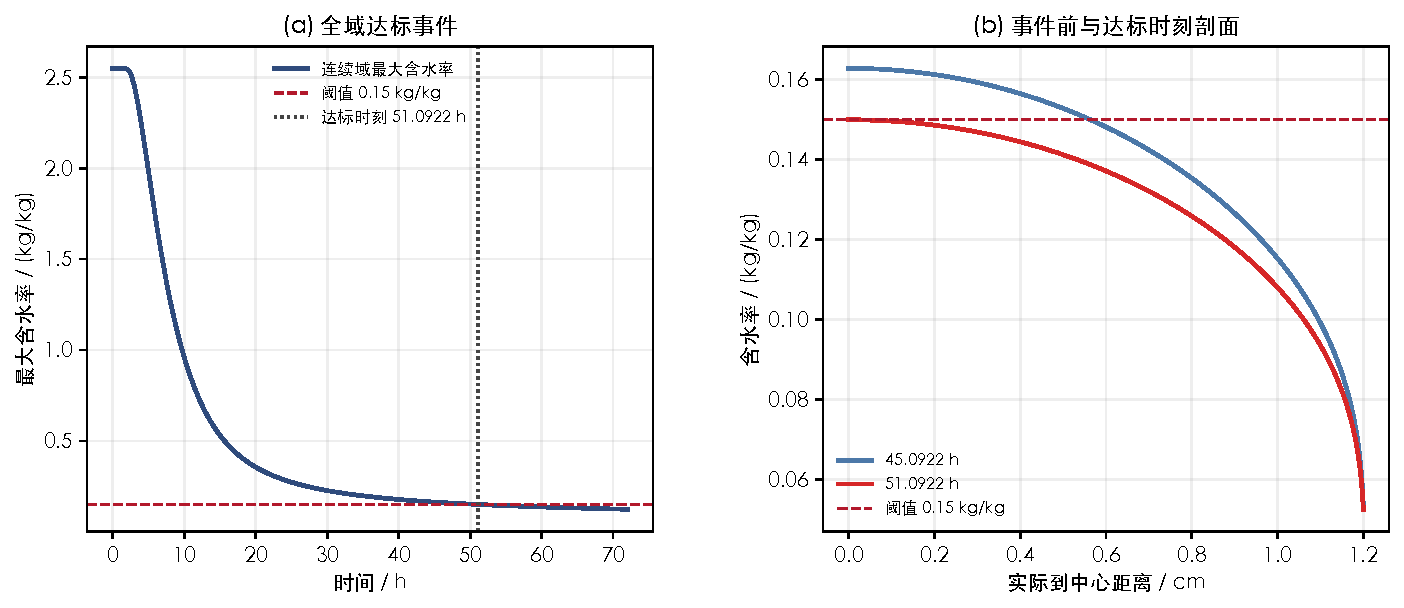
\includegraphics[width=0.98\textwidth]{../figures/q4/q4_shrink_event_combined.pdf}
  \caption{问题四连续域达标事件与收缩前后实际半径剖面}
  \label{fig:q4combined}
\end{figure}

\begin{figure}[H]
  \centering
  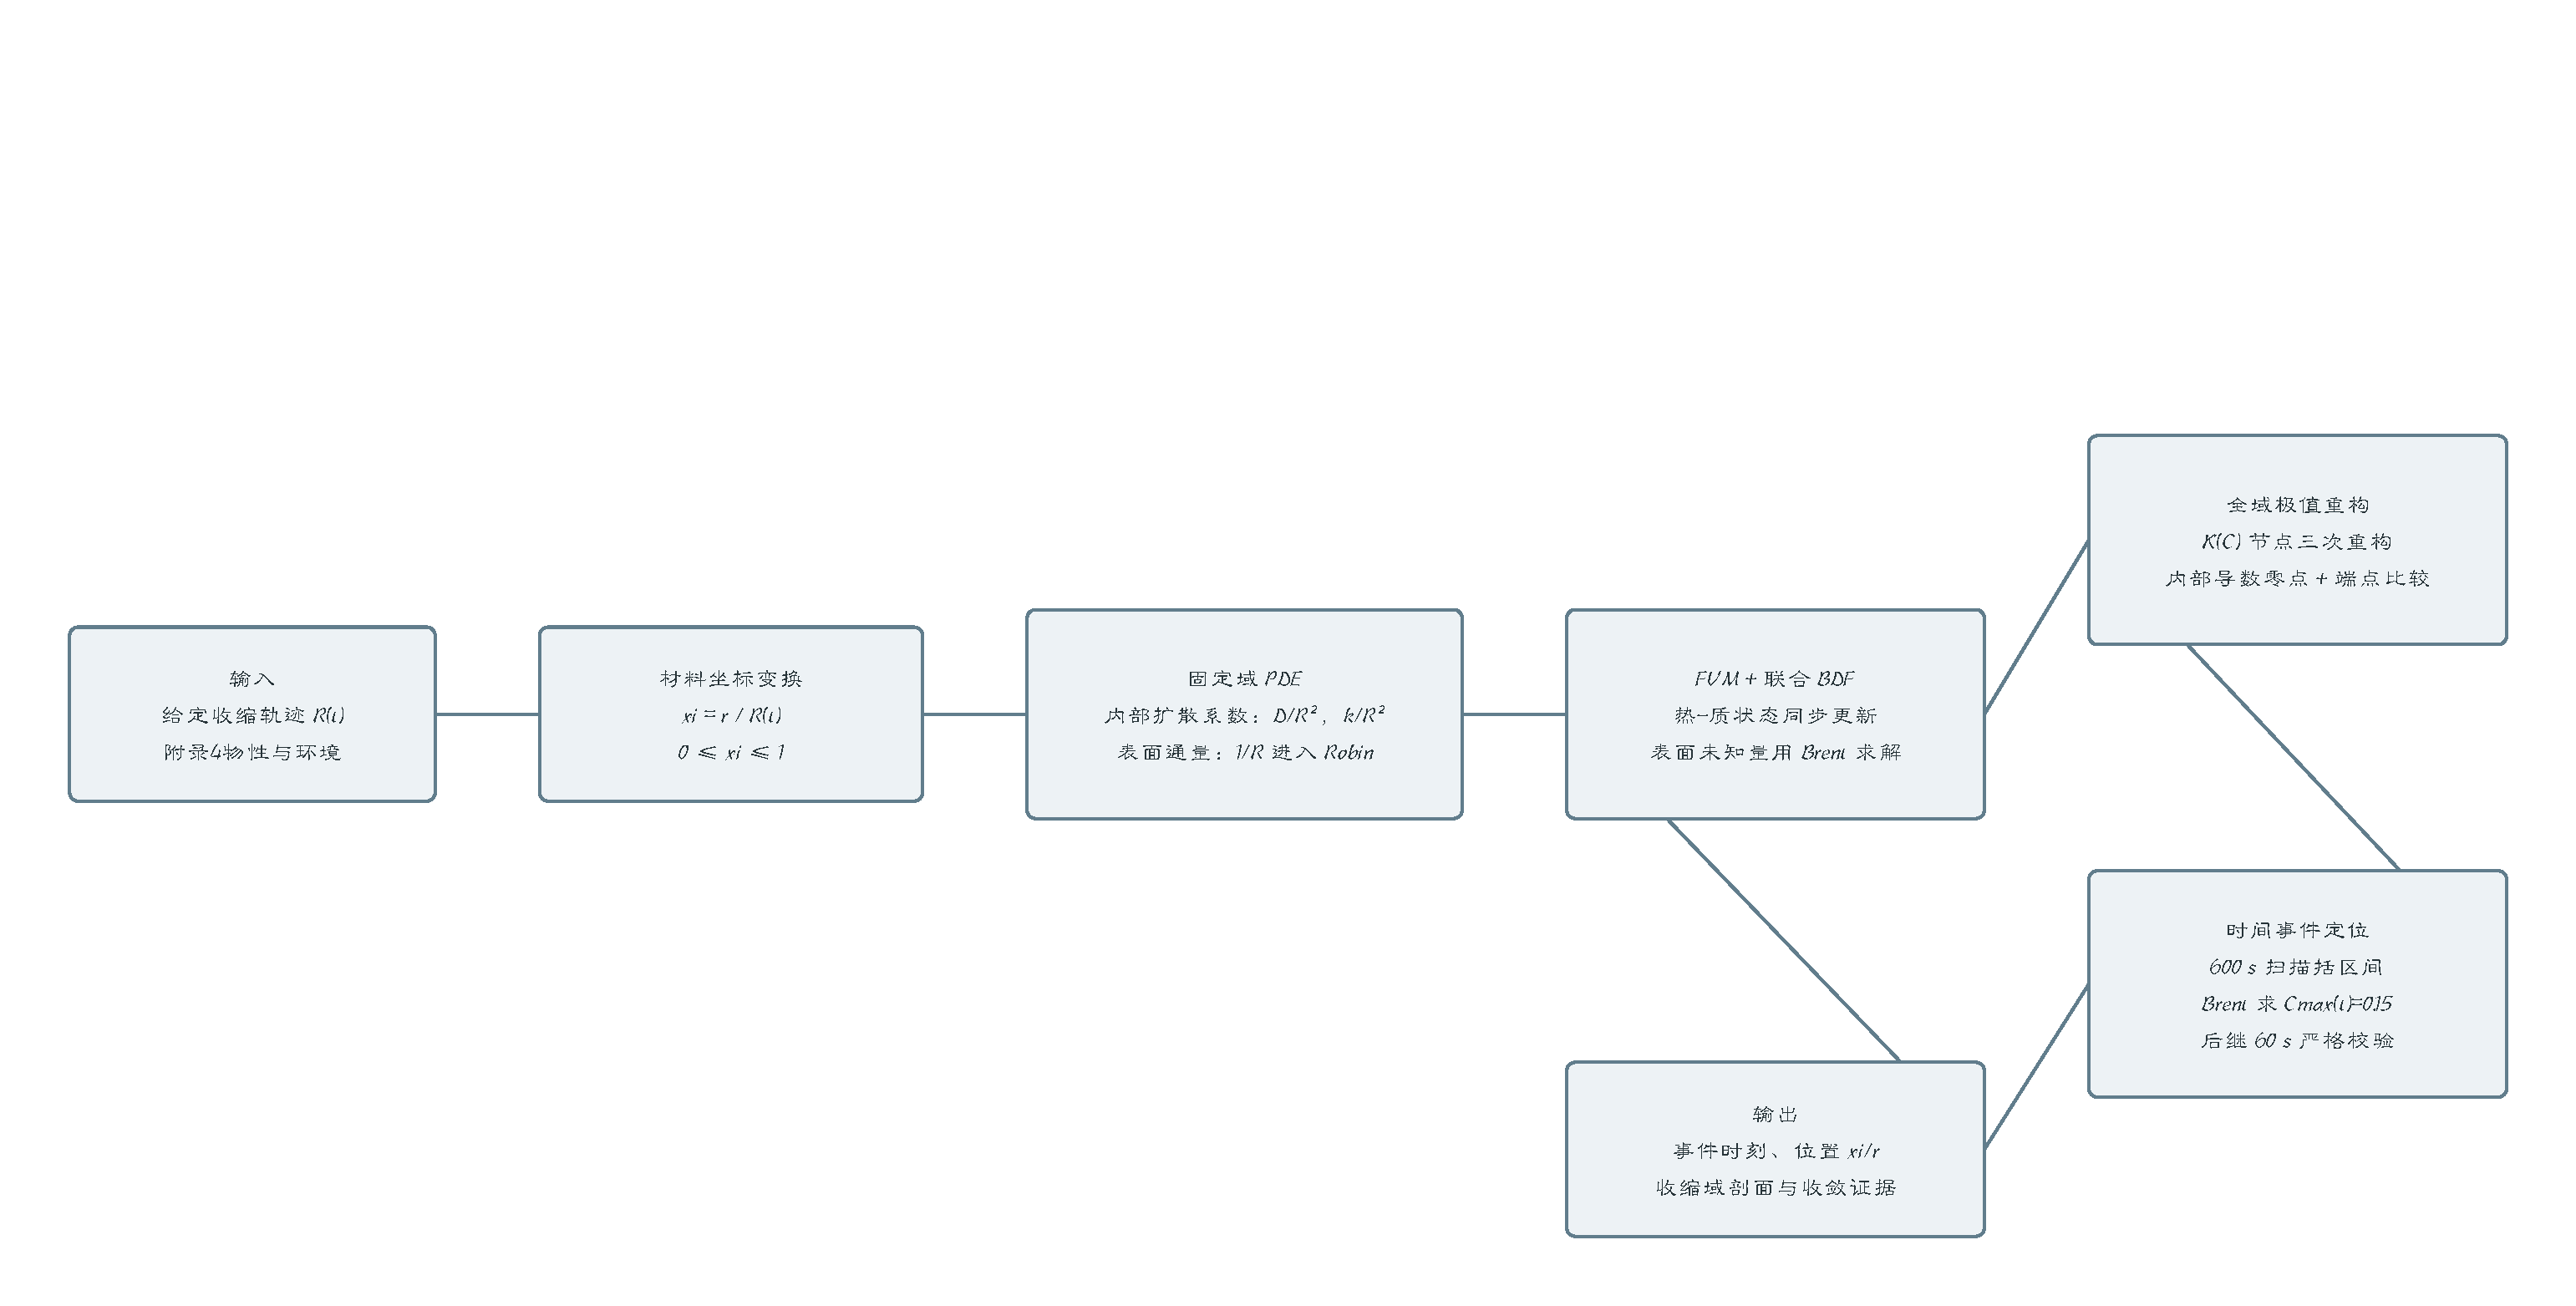
\includegraphics[width=0.82\textwidth]{../figures/q4/fig_q4_material_event.pdf}
  \caption{问题四材料坐标变换与事件定位流程}
  \label{fig:q4material}
\end{figure}

为区分几何和物性作用，设置固定/收缩半径与附录 3/4 的四种组合。达标时长分别为 57.47406473、129.84840533、25.24400627 和 51.09216535 h。顺序平均分解得到几何贡献 $-55.493149$ h、整组物性贡献 $49.111250$ h，交互贡献约 $-46.526182$ h，说明时长变化不能只归因于扩散率。
